\chapter{METODOLOGI}

% Ubah konten-konten berikut sesuai dengan isi dari metodologi
Berikut, pada gambar \ref{fig:blok-diagram}, adalah blok diagram dari penelitian yang dilakukan, 
yang secara besar terdiri dari 5 tahap.

\begin{figure}[H]
    \centering
    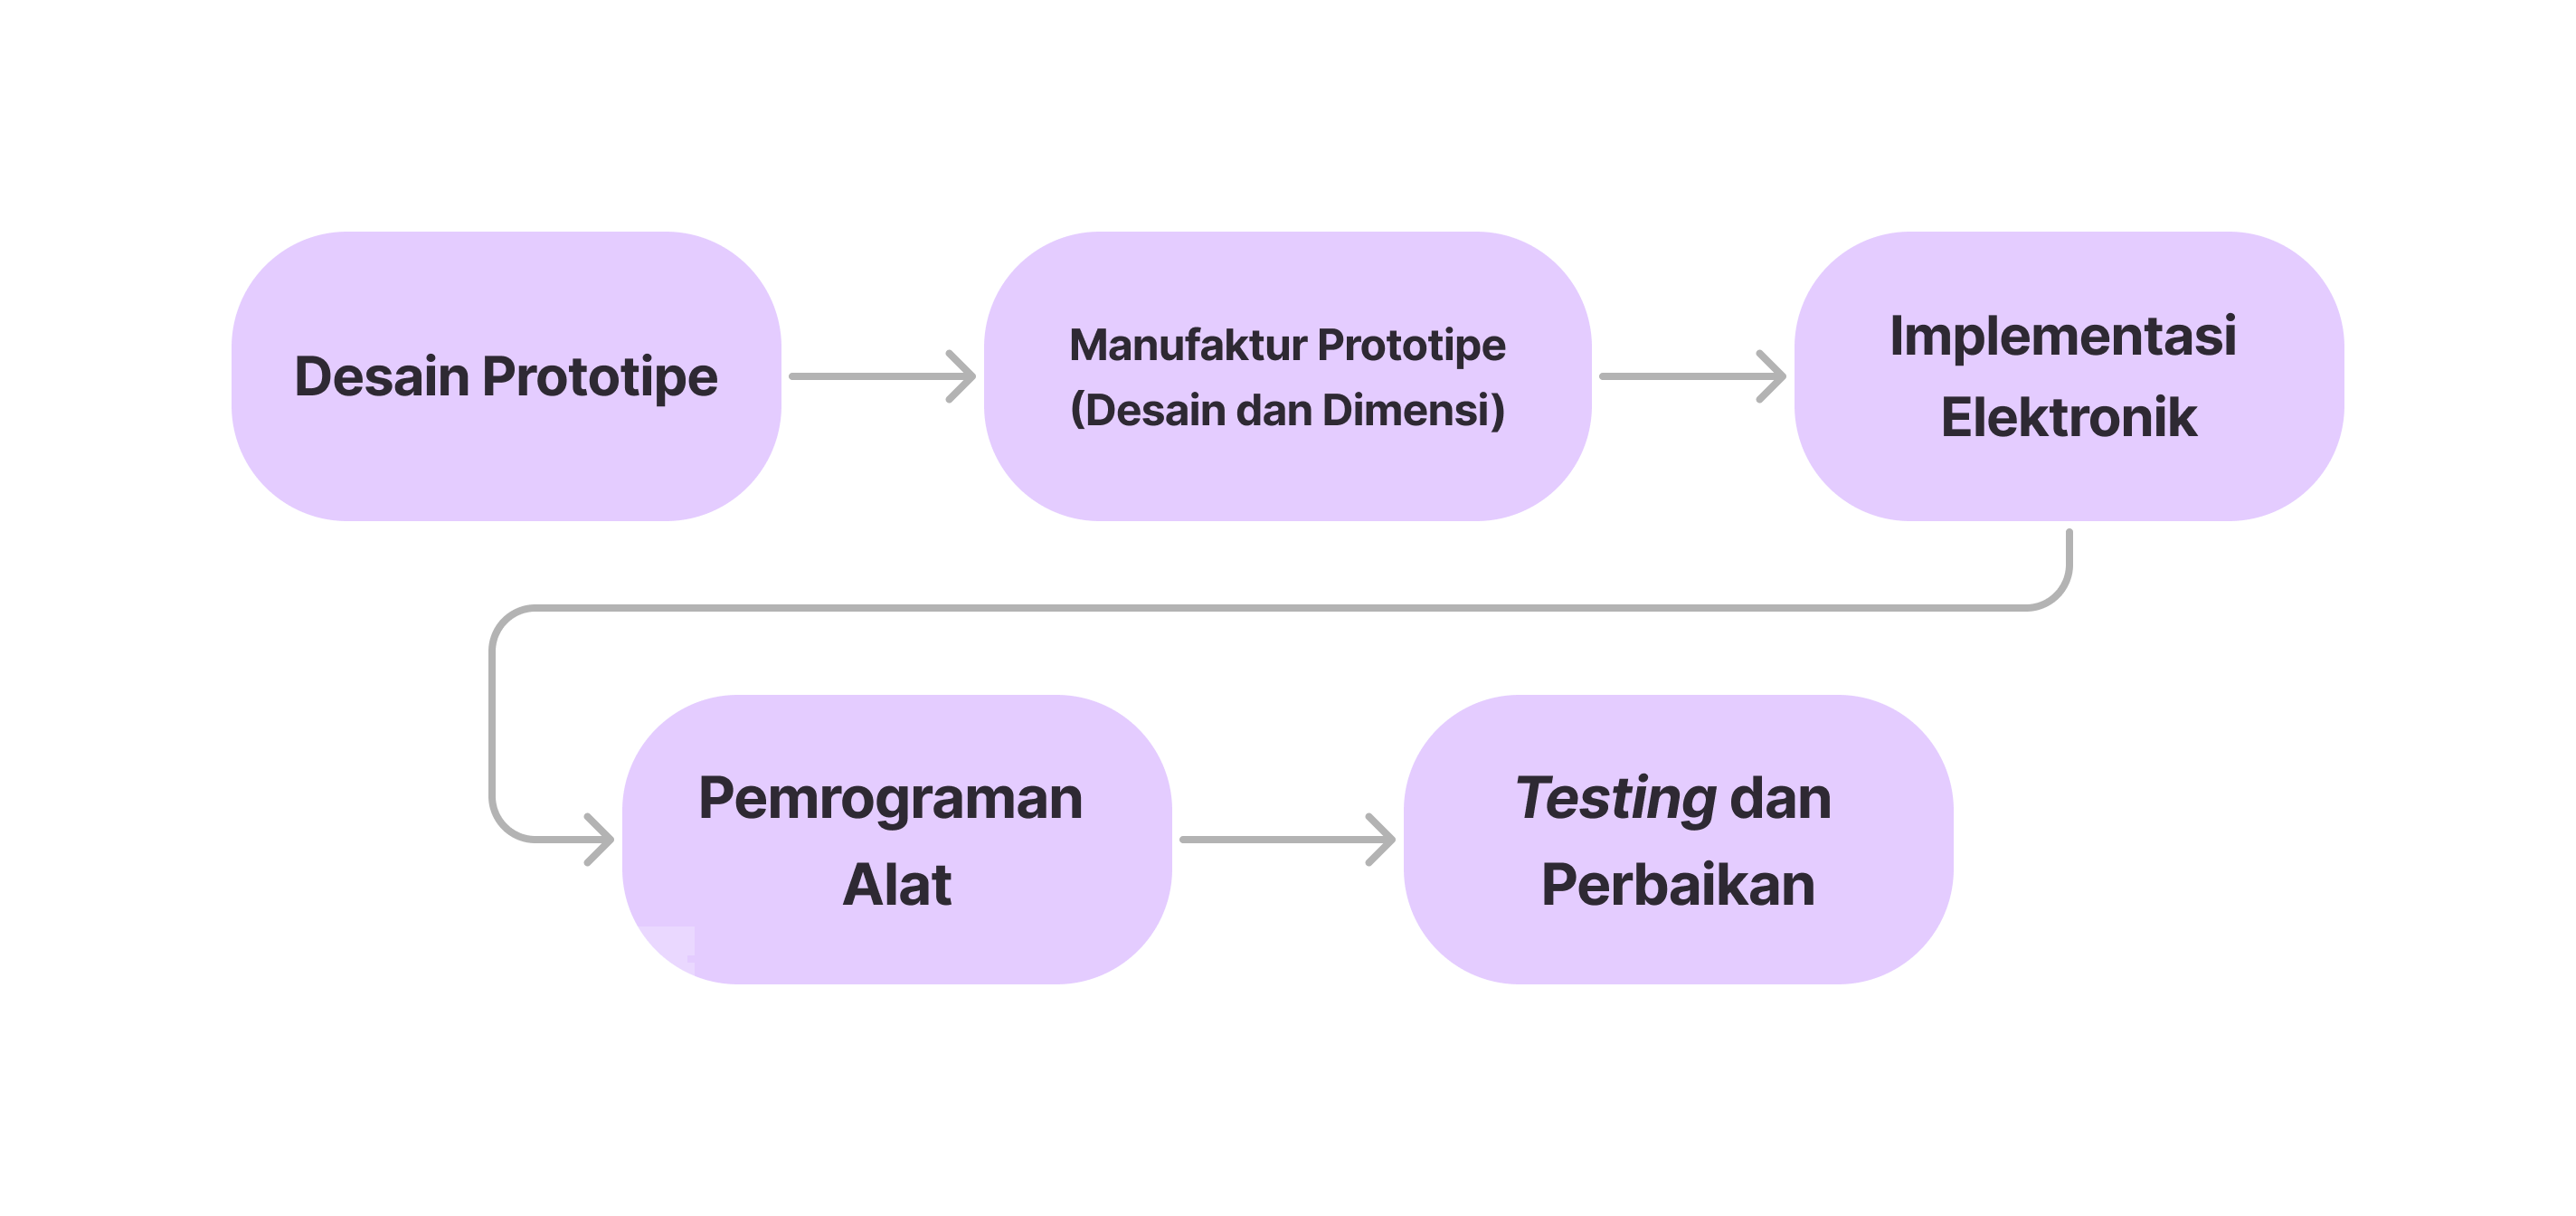
\includegraphics[width=1\linewidth]{gambar/diagram-metodologi.png}
    \caption{Blok Diagram Penelitian}
    \label{fig:blok-diagram}
\end{figure}

\section{Desain Prototipe}

Desain diawali dengan menggambar kasaran secara digital menggunakan \textit{software Goodnotes}
pada \textit{iPad}, memastikan desain yang akan dibuat sesuai dengan kebutuhan, fungsionalitas yang diinginkan,
dan ukuran yang sesuai.
Desain prototipe kemudian dilanjutkan dalam bentuk 3D \textit{Modelling} dengan 
bantuan \textit{software Computer Assisted Design} atau yang sering disebut 
sebagai \textit{CAD}. Aplikasi yang akan penulis gunakan dalam penelitian ini 
adalah \textit{Autodesk Fusion 360}. Dengan \textit{software} ini, penulis dapat menghasilkan gambar
teknik yang lebih rinci dan detail, sehingga dapat dijadikan acuan dalam proses manufaktur.
Juga software ini dapat melakukan export file dalam format \textit{.stl} yang dapat digunakan
dalam proses manufaktur menggunakan \textit{3D Printer}.

Ada beberapa desain yang telah dibuat, sesuai pada gambar \ref{fig:desain-prototipe-2} dan gambar 
\ref{fig:desain-prototipe-3}, desain ini dibuat sehingga dapat 
menyesuaikan dengan meteran listrik prabayar yang biasa terpasang di rumah-rumah secara 
\textit{universal}. Dengan desain yang menggunakan \textit{clamp} sehingga dapat menyesuaikan dengan
ukuran alat meteran listrik prabayar yang berbeda-beda.

\begin{figure}[H]
    \centering
    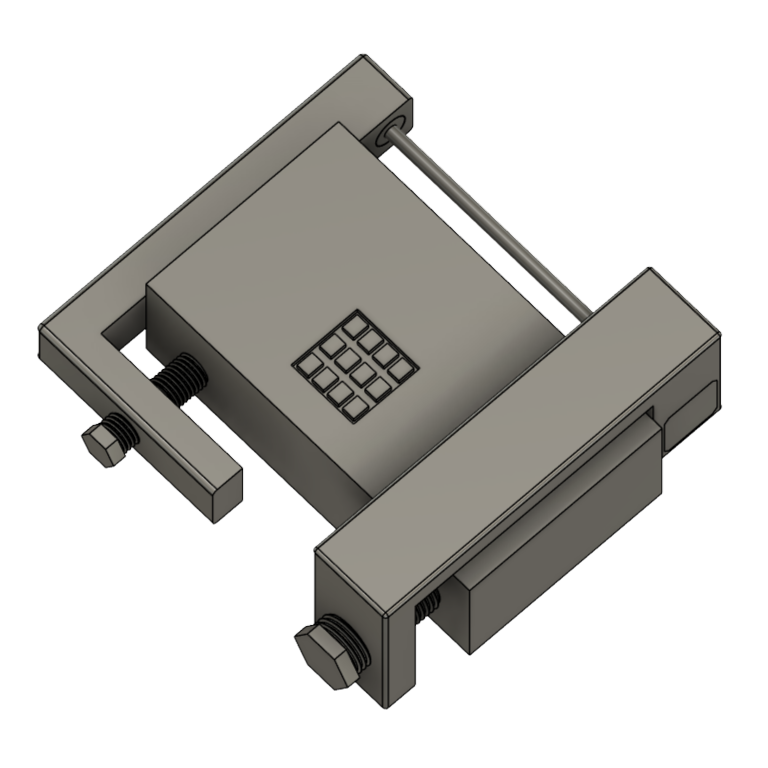
\includegraphics[width=0.4\linewidth]{gambar/prototype-2.png}
    \caption{Desain Prototipe Pertama}
    \label{fig:desain-prototipe-2}
\end{figure}

\begin{figure}[H]
  \centering
  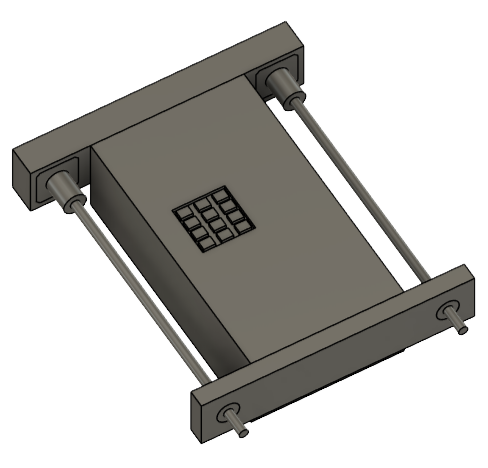
\includegraphics[width=0.4\linewidth]{gambar/prototype-3.png}
  \caption{Desain Prototipe Kedua}
  \label{fig:desain-prototipe-3}
\end{figure}

Desain diatas merupakan protipe yang belum final, dimana masih memerlukan beberapa perbaikan, 
juga bagian pergerakan horizontal (sumbu-x) masih belum diimplementasikan.

\section{Manufaktur Prototipe}

Manufaktur prototipe dilakukan menggunakan bantuan \textit{3D Printer} dengan merek 
\textit{Bambulab A1}. Penulis menggunakan \textit{3D Printer} ini karena dilengkapi dengan fitur yang
sangat lengkap, beberapa dari fitur tersebut adalah
sistem \textit{AMS Lite} yaitu merupakan sistem yang dapat mengatur perubahan material yang digunakan
secara lebih mudah sehingga dapat menggabungkan beberapa material atau warna yang berbeda dalam satu cetakan,
kemudian ada fitur \textit{Auto Bed Leveling} yang dapat mengatur keseimbangan \textit{bed plate} 
dari \textit{3D Printer} secara otomatis memastikan cetakan yang dihasilkan lebih rata dan presisi.
Fitur lainnya yang sangat membantu dalam manufaktur adalah beberapa sensor yang terpasang pada \textit{3D Printer},
beberapanya adalah sensor \textit{filament runout} yang dapat memberikan notifikasi ketika \textit{filament},
habis, kemudian sensor \textit{filament tangle} yang dapat memberikan notifikasi ketika \textit{filament}
terjebak atau terlilit, dan masih banyak lagi fitur lainnya.
Fitur - fitur tersebut sangat membantu dalam proses manufaktur prototipe yang butuh pengulangan
yang cukup banyak, sehingga penulis dapat memfokuskan waktu pada tahap desain dan pengujian.

Proses manufaktur diawali dengan menghasilkan file \textit{.stl} dari desain yang telah dibuat menggunakan \textit{Autodesk Fusion 360}, ke- mudian
file tersebut diolah menggunakan \textit{software Slicer}, sesuai pada gambar \ref{fig:bambu-studio},
yang memotong model 3D menjadi beberapa lapisan dan menyatakan perintah sehingga dapat dicetak oleh \textit{3D Printer}. 
Penulis menggunakan \textit{software Bambu Studio} yang dapat diakses melalui \textit{cloud} yang 
terhubung dengan \textit{3D Printer}. File \textit{.stl} tersebut merupakan representasi dari objek 3 dimensi yang dibuat dari lapisan-lapisan
2 dimensi, yang dimana dijadikan sebagai acuan sesuai dengan lokasi tertentu oleh \textit{3D Printer} 
untuk mencetak objek tersebut. Kemudian file tersebut diunggah ke \textit{cloud} yang terhubung dengan
\textit{3D Printer}, kemudian \textit{3D Printer} akan membaca file tersebut dan mencetak objek tersebut.

\begin{figure}[H]
  \centering
  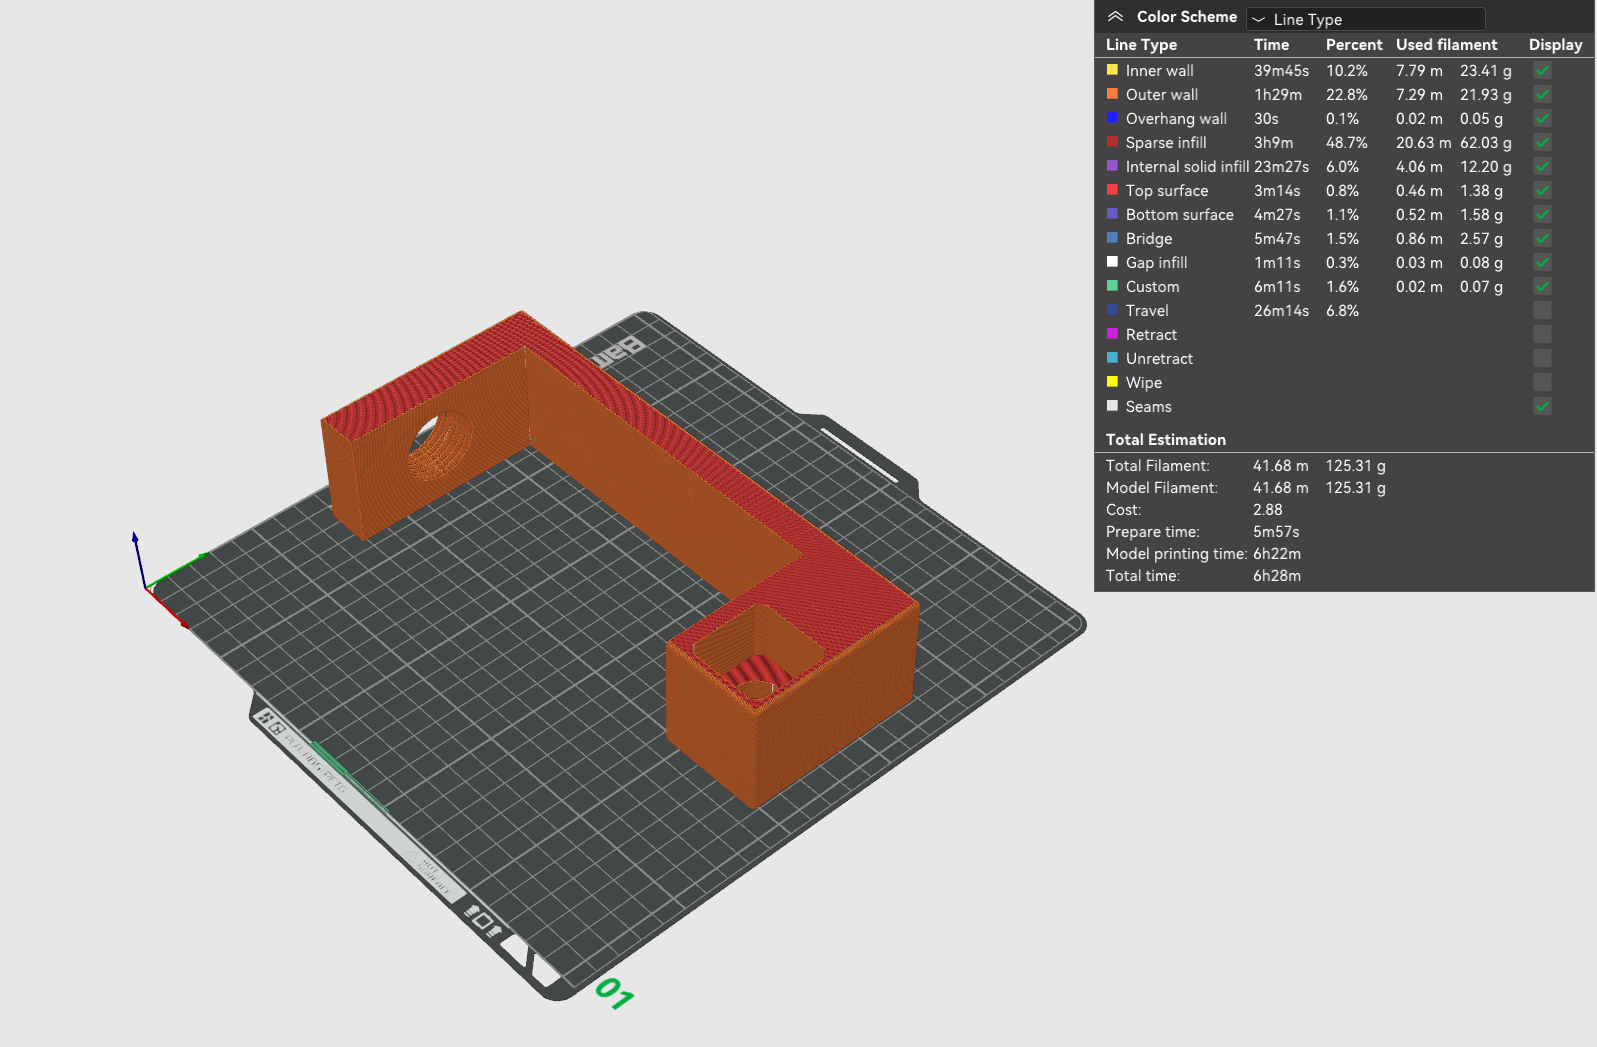
\includegraphics[width=0.7\linewidth]{gambar/bambu-studio.png}
  \caption{file \textit{.stl} yang diolah menggunakan \textit{software Slicer}}
  \label{fig:bambu-studio}
\end{figure}

Hasil dari manufaktur prototipe dan implementasinya tertera pada gambar \ref{fig:hasil-prototipe-1}, dimana prototipe tersebut masih dalam tahap pengujian 
dan perbaikan, namun dapat menjadi visualisasi dan representasi yang baik untuk hasil produk akhir. Material yang digunakan dalam manufaktur prototipe adalah \textit{PLA} atau \textit{Polylactic Acid},
material ini digunakan karena harga nya yang terjangkau, mudah dicetak, dan cukup kuat untuk digunakan
sebagai prototipe. Namun, material ini memiliki kekurangan yaitu tidak tahan terhadap panas dan
suhu tinggi, sehingga tidak dapat digunakan dalam lingkungan yang memiliki suhu tinggi. Sebagai 
alternatif material yang digunakan adalah \textit{PETG} atau \textit{Polyethylene Terephthalate Glycol},
material ini memiliki kelebihan yaitu tahan terhadap suhu tinggi, kuat, dan tahan terhadap benturan,
namun material ini memiliki harga yang lebih mahal dibandingkan \textit{PLA} dan lebih sulit untuk
dicetak.

\begin{figure}[H]
  \centering
  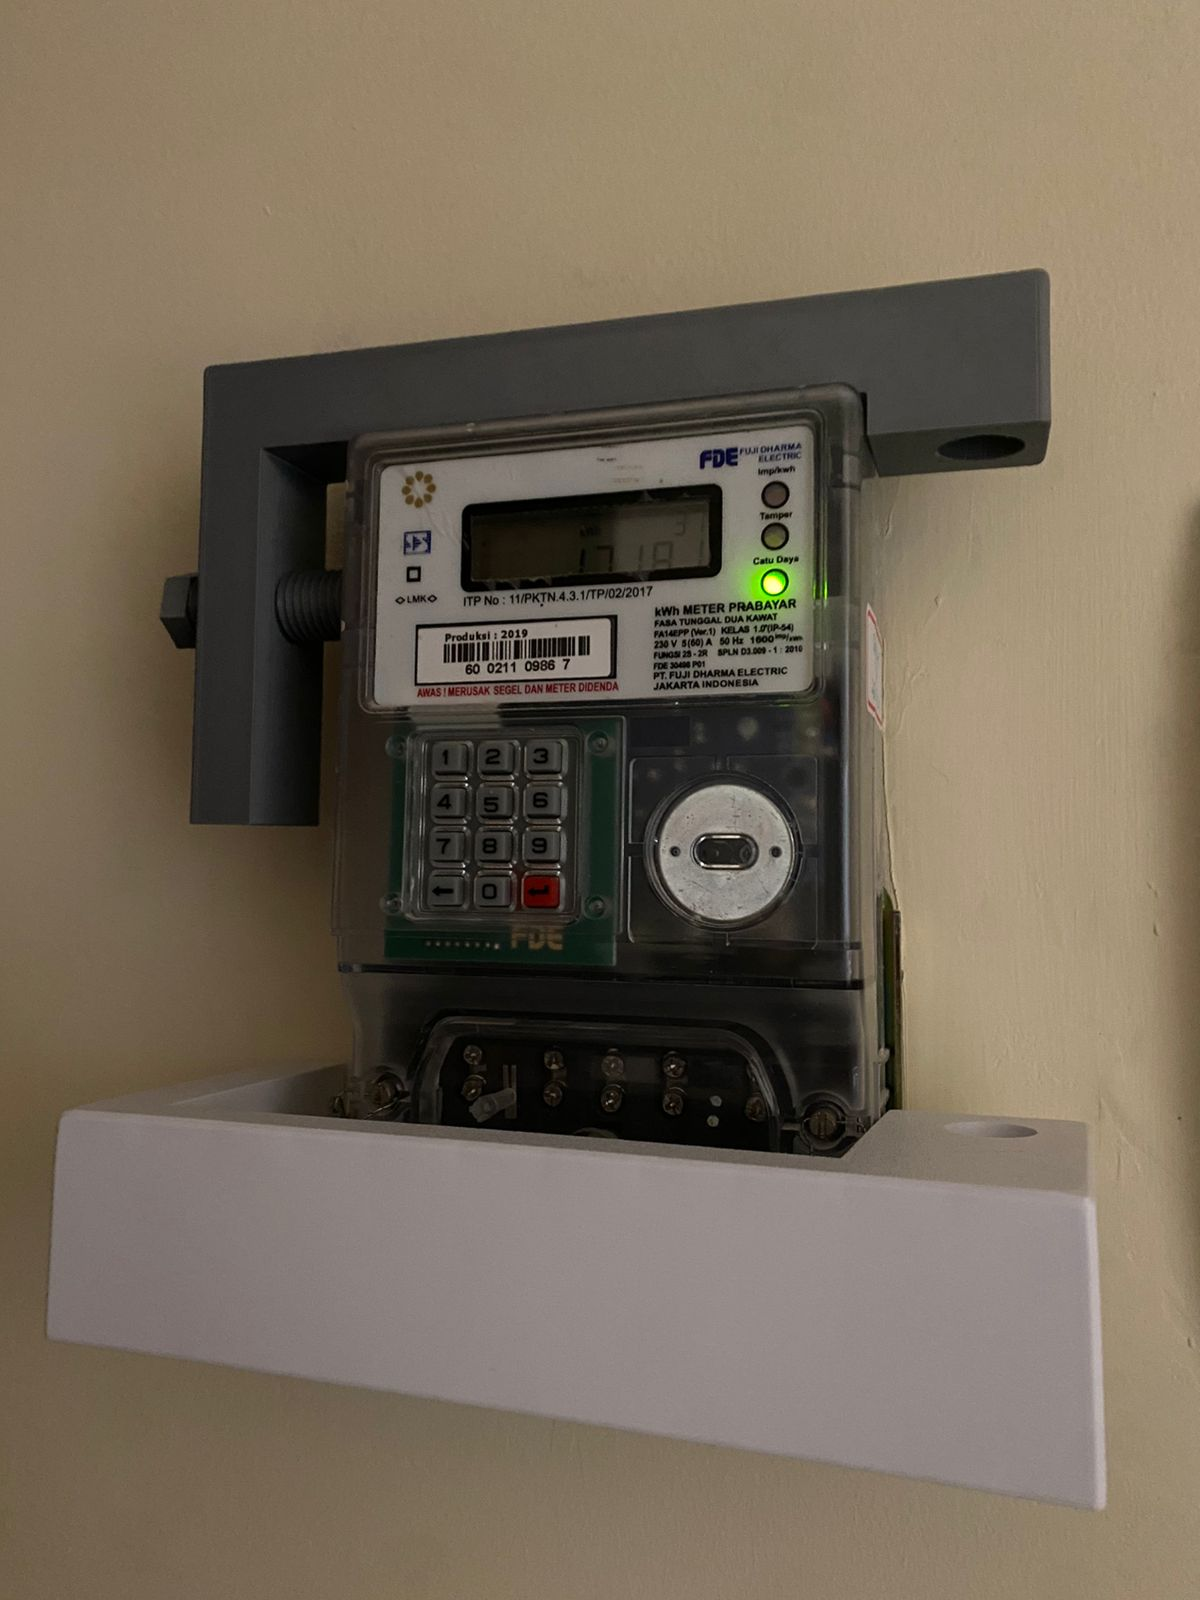
\includegraphics[width=0.4\linewidth]{gambar/contoh-prototipe-kerangka.jpg}
  \caption{Contoh manufaktur prototipe menggunakan \textit{3D Printer}}
  \label{fig:hasil-prototipe-1}
\end{figure}

\section{Implementasi Elektronik}

\begin{figure}[H]
  \centering
  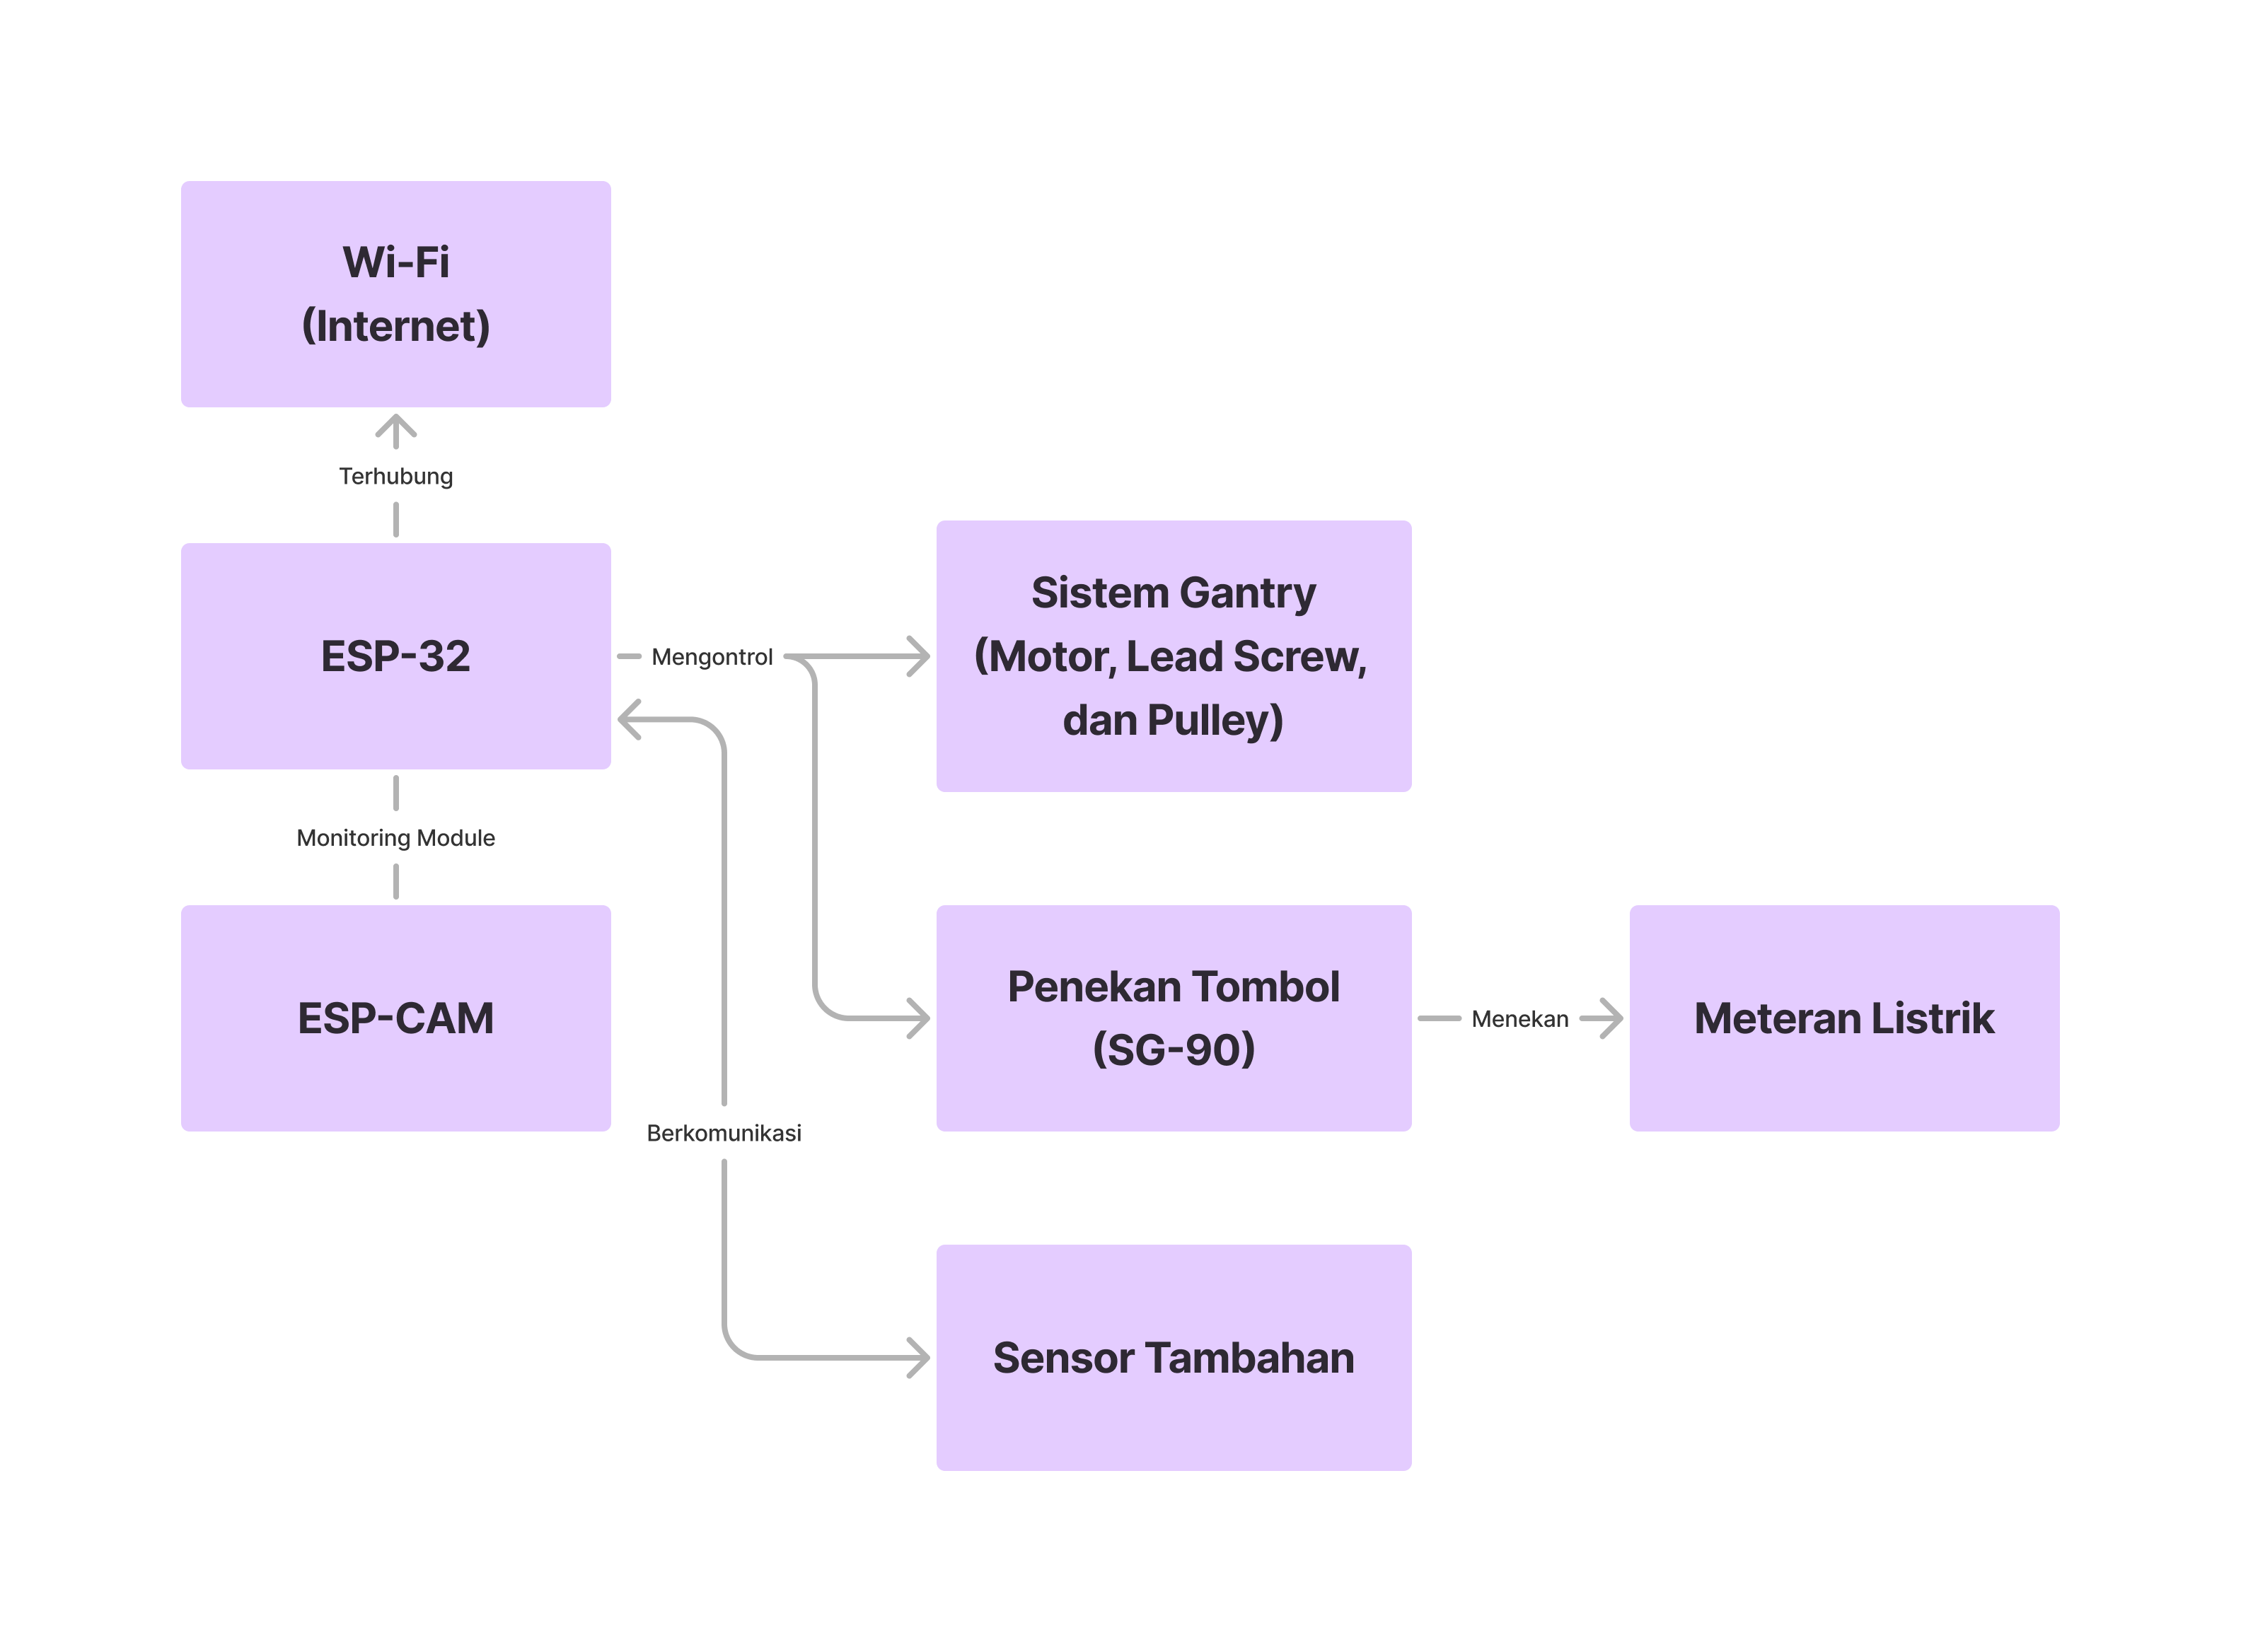
\includegraphics[width=1\linewidth]{gambar/implementasi-elektronik.png}
  \caption{Diagram hubungan komponen elektronik}
  \label{fig:implementasi-elektronik}
\end{figure}

Ada beberapa komponen elektronik yang digunakan dalam penelitian ini sesuai pada gambar \ref{fig:implementasi-elektronik},
beberapa diantaranya adalah
mikrokontoler \textit{ESP32} akan diprogram untuk menjalankan seluruh pergerakan dari alat, baik dari
pergerakan vertikal, horizontal, maupun penekanan tombol dari meteran listrik. \textit{ESP32} juga akan
terhubung ke internet melalui Wi-Fi sehingga pengguna dapat mengontrol alat dari jarak jauh. 
Kemudian motor yang digunakan
adalah motor \textit{stepper} NEMA-14 untuk pergerakan horizontal dan vertikal yang dikontrol menggunakan
\textit{motor driver} DRV8825, motor ini digunakan karena
ukurannya yang kecil dan cukup kuat untuk menggerakkan alat, salah satu motor tersebut akan dihubungkan
ke \textit{lead-screw} dan sekrupnya yang juga dibantu dengan \textit{guide rail} MGN12, 
yang menjadi penggerak vertikal utama dari alat, dan motor lainnya
akan terhubung ke sistem \textit{pulley} yang menjadi penggerak horizontal dari alat. kemudian motor 
\textit{servo} SG-90 untuk penekanan tombol pada meteran listrik, motor ini digunakan karena ukurannya 
yang kecil dan cukup kuat dengan \textit{torque} 1.98 kg/cm. 
Kemudian akan digunakan juga ESP-CAM sebagai sarana monitoring jarak jauh
dari alat, ESP-CAM ini digunakan karena kemampuannya yang dapat mengirimkan 
data melalui jaringan \textit{Wi-Fi}.
Penulis juga berencana untuk menggunakan beberapa sensor tambahan, seperti sensor jarak ultrasonik,
yang difungsikan sebagai sarana kalibrasi dan pengukuran jarak dari alat ke meteran listrik,
memastikan penggunaan alat dapat akurat dan presisi. Namun, sensor ini masih dalam tahap pengujian
sehingga belum diimplementasikan dalam prototipe. Kemudian baterai lithium-ion akan digunakan sebagai
sumber daya dari alat, sehingga alat dapat dipasang secara portabel tanpa perlu terhubung ke sumber listrik AC.

\section{Pemrograman Alat}

\begin{figure}[H]
  \centering
  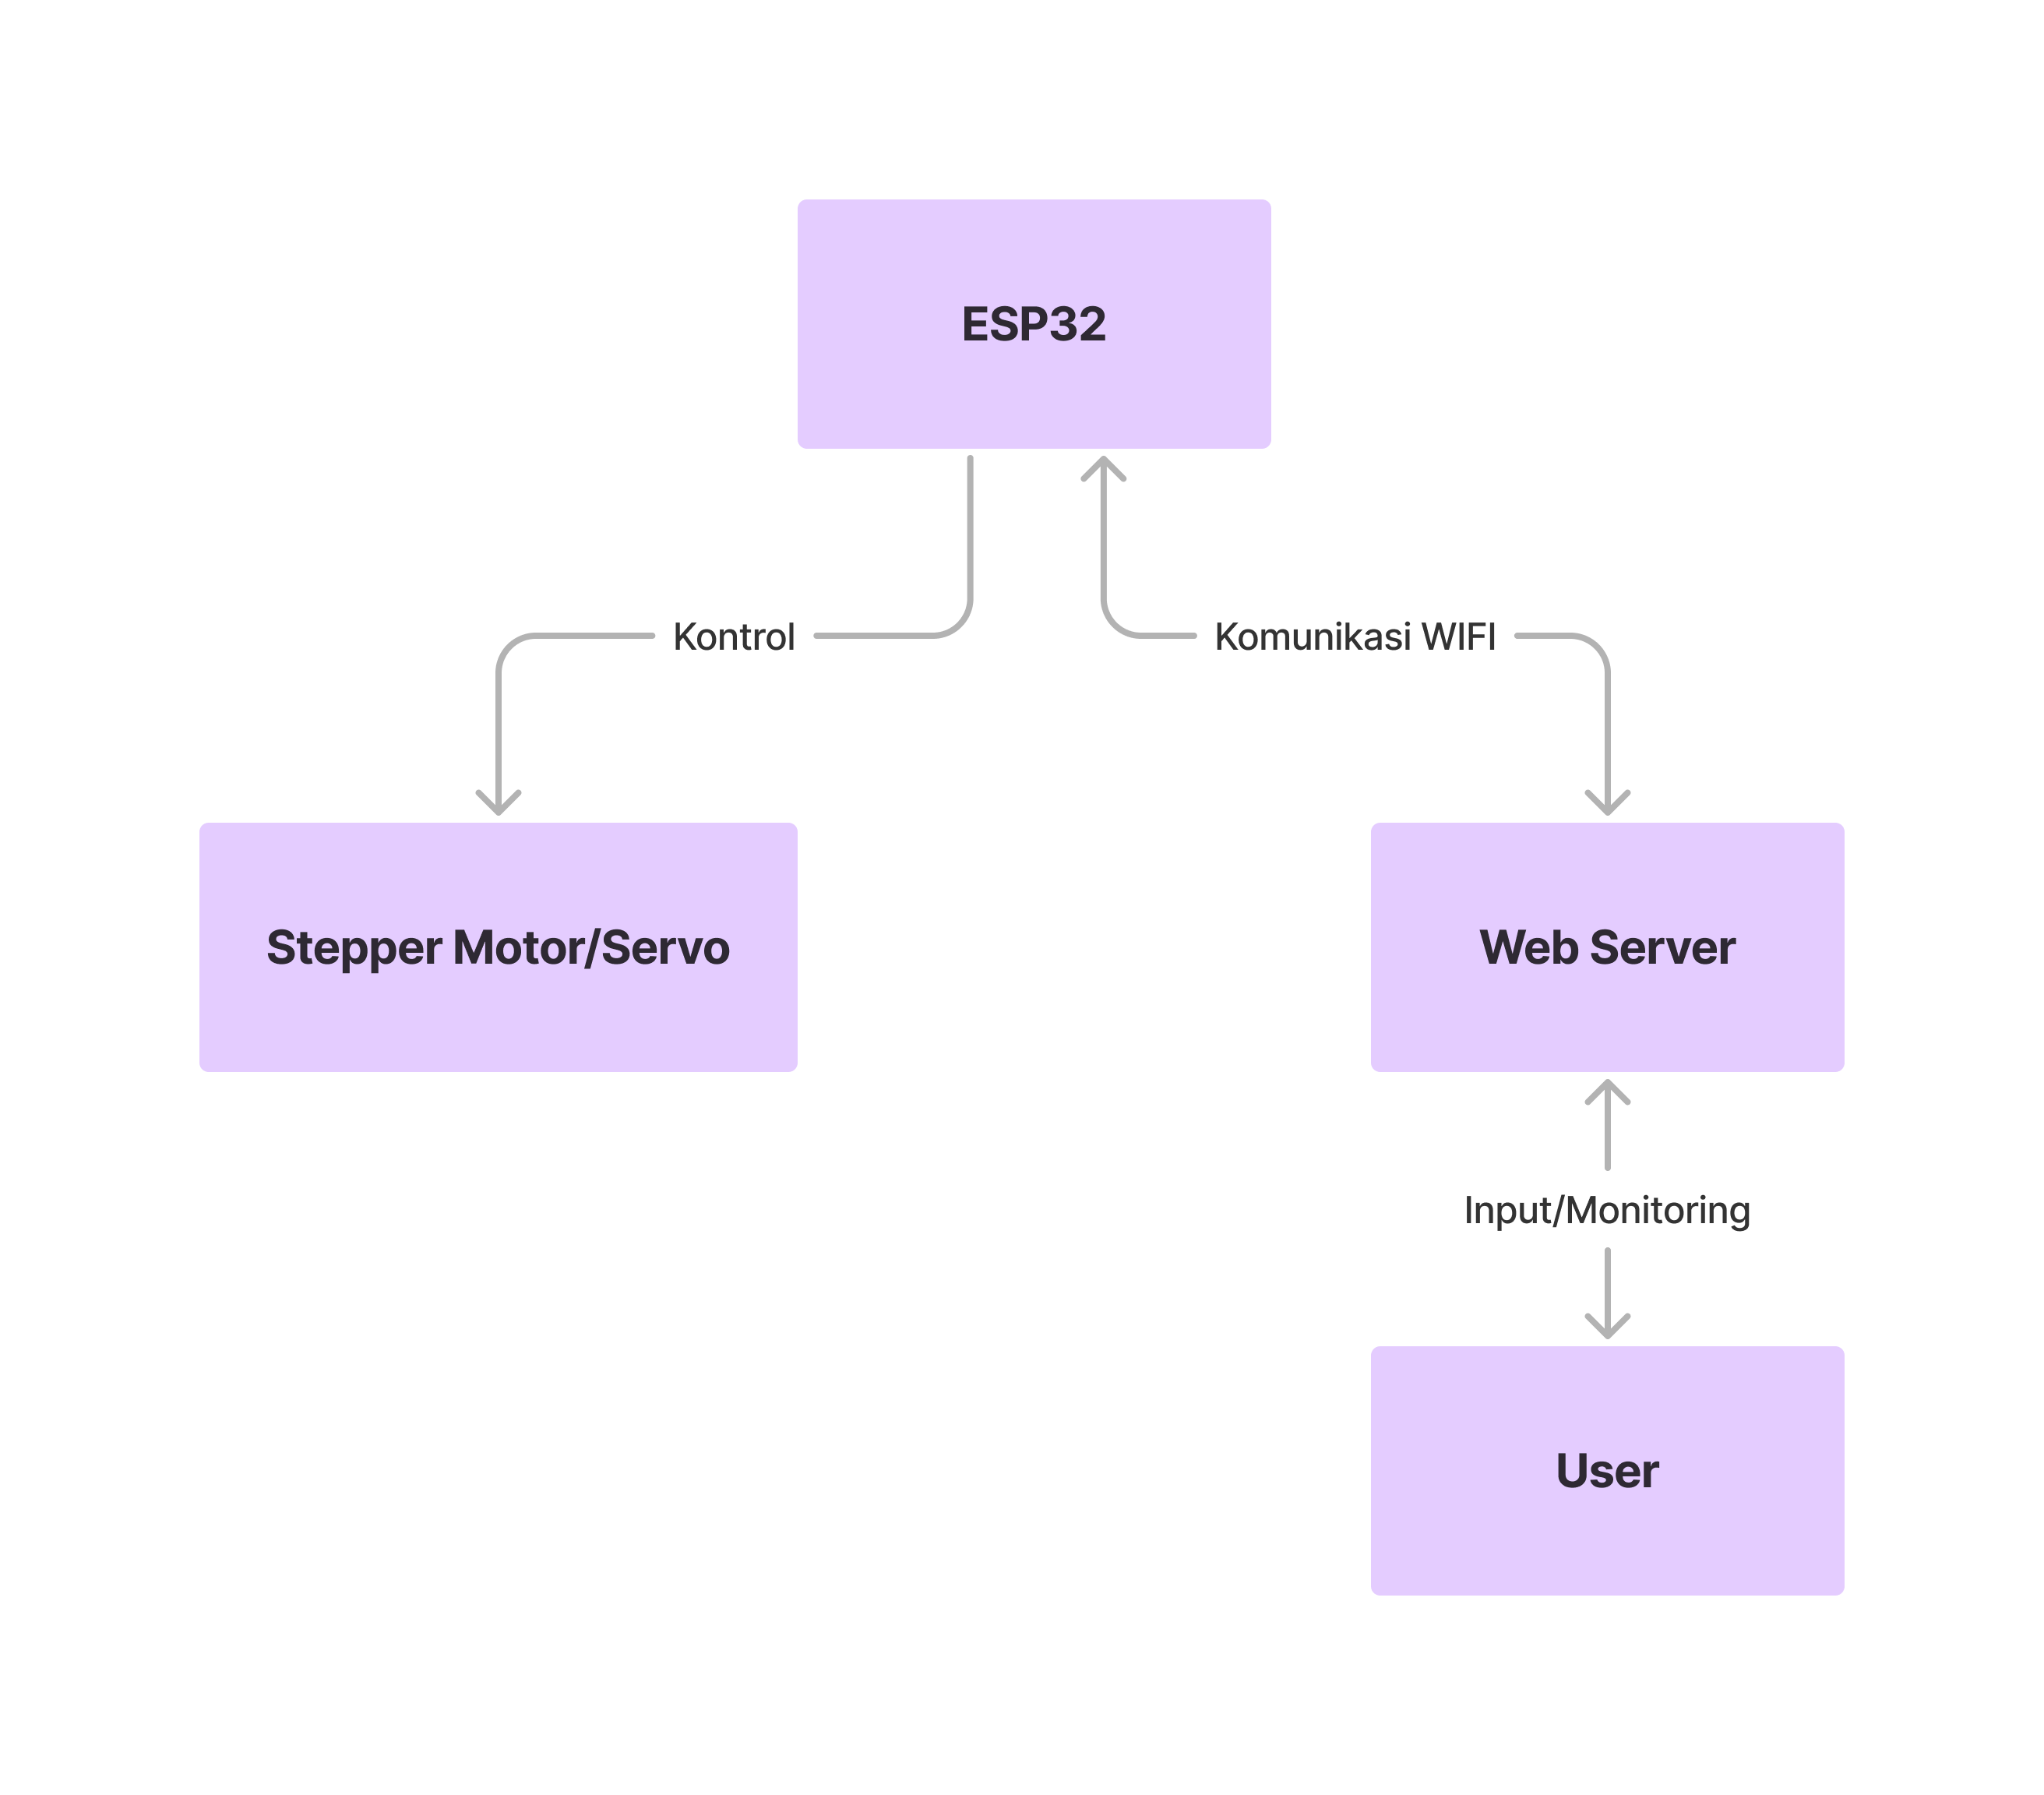
\includegraphics[width=0.8\linewidth]{gambar/diagram-program.png}
  \caption{Diagram hubungan program alat}
  \label{fig:diagram-program}
\end{figure}

Pemrograman alat dilakukan dengan menggunakan \textit{Arduino IDE} langsung menuju ESP32, kemudian komponen listrik
seperti motor stepper dan servo akan diatur menggunakan \textit{library} yang sudah disediakan oleh \textit{Arduino IDE}.
Beberapa dari \textit{library} yang digunakan adalah \textit{AccelStepper.h} untuk motor stepper (yang terhubung ke driver motor), 
\textit{Servo.h} untuk motor servo, dan \textit{WiFi.h} untuk koneksi internet. 

Secara garis besar,
algoritma yang digunakan diawali dengan memastikan koneksi internet terhubung dan dapat berkomunikasi dengan
\textit{web interface}, kemudian dilakukan
kalibrasi dari motor stepper dan servo memastikan jarak maksimum dari masing masing motor dan posisi
angka dari meteran listrik, untuk kalibrasi pergerakan vertikal dan horizontal dapat digunakan tombol yang menentukan titik
maksimum dan minimum dari posisi alat, sedangkan kalibrasi posisi tombol dapat dilakukan dari \textit{web interface} secara manual,
memastikan alat dapat digunakan di berbagai meteran listrik prabayar.
kemudian pengguna memberikan input melalui \textit{web interface}/aplikasi yang terhubung ke ESP32,
dan ESP32 akan menggerakkan motor stepper dan servo sesuai dengan input yang diberikan.

\textit{Web interface} dari alat berisikan dua fungsi utama, yaitu input dan monitoring, pada bagian input user dapat memasukkan
token yang telah mereka beli, kemudian input tersebut akan dikirimkan melalui jaringan internet ke ESP32, kemudian ESP32 akan
menggerakkan motor servo untuk menekan tombol pada meteran listrik, kemudian pada bagian monitoring, user dapat melihat menggunakan
kamera yang terpasang pada ESP32 untuk memastikan bahwa alat berfungsi dengan baik dan dapat melihat sisa kWh yang tersisa pada meteran listrik.

\section{\textit{Testing} dan Perbaikan}

Setelah alat atau prototipe alat selesai dibuat, dilakukan \textit{testing} untuk memastikan alat dapat berfungsi sesuai dengan
yang diinginkan, beberapa tes yang dilakukan adalah memastikan bahwa alat dapat bergerak secara vertikal dan horizontal dengan baik
dan mulus, kemudian memastikan bahwa kalibrasi dari alat dapat berjalan dengan baik. Alat juga harus dipastikan dapat menekan tombol
dengan akurat dalam banyak percobaan sehinga dapat digunakan dalam jangka waktu yang lama tanpa perlu banyak perbaikan atau kalibrasi ulang.
Kemudian alat juga harus dipastikan dapat berkomunikasi dengan \textit{web interface} dengan baik, sehingga pengguna dapat melakukan
input dan monitoring tanpa ada gangguan. Jika terdapat kesalahan atau kekurangan, maka dilakukan perbaikan dan pengulangan dari tahap
\textit{testing} hingga alat dapat berfungsi dengan baik sesuai dengan tujuan dari penelitian.
